\documentclass[]{article}
\usepackage{lmodern}
\usepackage{amssymb,amsmath}
\usepackage{ifxetex,ifluatex}
\usepackage{fixltx2e} % provides \textsubscript
\ifnum 0\ifxetex 1\fi\ifluatex 1\fi=0 % if pdftex
  \usepackage[T1]{fontenc}
  \usepackage[utf8]{inputenc}
\else % if luatex or xelatex
  \ifxetex
    \usepackage{mathspec}
  \else
    \usepackage{fontspec}
  \fi
  \defaultfontfeatures{Ligatures=TeX,Scale=MatchLowercase}
\fi
% use upquote if available, for straight quotes in verbatim environments
\IfFileExists{upquote.sty}{\usepackage{upquote}}{}
% use microtype if available
\IfFileExists{microtype.sty}{%
\usepackage{microtype}
\UseMicrotypeSet[protrusion]{basicmath} % disable protrusion for tt fonts
}{}
\usepackage[margin=1in]{geometry}
\usepackage{hyperref}
\hypersetup{unicode=true,
            pdftitle={meeting report 5.27},
            pdfauthor={linyiguo},
            pdfborder={0 0 0},
            breaklinks=true}
\urlstyle{same}  % don't use monospace font for urls
\usepackage{color}
\usepackage{fancyvrb}
\newcommand{\VerbBar}{|}
\newcommand{\VERB}{\Verb[commandchars=\\\{\}]}
\DefineVerbatimEnvironment{Highlighting}{Verbatim}{commandchars=\\\{\}}
% Add ',fontsize=\small' for more characters per line
\usepackage{framed}
\definecolor{shadecolor}{RGB}{248,248,248}
\newenvironment{Shaded}{\begin{snugshade}}{\end{snugshade}}
\newcommand{\AlertTok}[1]{\textcolor[rgb]{0.94,0.16,0.16}{#1}}
\newcommand{\AnnotationTok}[1]{\textcolor[rgb]{0.56,0.35,0.01}{\textbf{\textit{#1}}}}
\newcommand{\AttributeTok}[1]{\textcolor[rgb]{0.77,0.63,0.00}{#1}}
\newcommand{\BaseNTok}[1]{\textcolor[rgb]{0.00,0.00,0.81}{#1}}
\newcommand{\BuiltInTok}[1]{#1}
\newcommand{\CharTok}[1]{\textcolor[rgb]{0.31,0.60,0.02}{#1}}
\newcommand{\CommentTok}[1]{\textcolor[rgb]{0.56,0.35,0.01}{\textit{#1}}}
\newcommand{\CommentVarTok}[1]{\textcolor[rgb]{0.56,0.35,0.01}{\textbf{\textit{#1}}}}
\newcommand{\ConstantTok}[1]{\textcolor[rgb]{0.00,0.00,0.00}{#1}}
\newcommand{\ControlFlowTok}[1]{\textcolor[rgb]{0.13,0.29,0.53}{\textbf{#1}}}
\newcommand{\DataTypeTok}[1]{\textcolor[rgb]{0.13,0.29,0.53}{#1}}
\newcommand{\DecValTok}[1]{\textcolor[rgb]{0.00,0.00,0.81}{#1}}
\newcommand{\DocumentationTok}[1]{\textcolor[rgb]{0.56,0.35,0.01}{\textbf{\textit{#1}}}}
\newcommand{\ErrorTok}[1]{\textcolor[rgb]{0.64,0.00,0.00}{\textbf{#1}}}
\newcommand{\ExtensionTok}[1]{#1}
\newcommand{\FloatTok}[1]{\textcolor[rgb]{0.00,0.00,0.81}{#1}}
\newcommand{\FunctionTok}[1]{\textcolor[rgb]{0.00,0.00,0.00}{#1}}
\newcommand{\ImportTok}[1]{#1}
\newcommand{\InformationTok}[1]{\textcolor[rgb]{0.56,0.35,0.01}{\textbf{\textit{#1}}}}
\newcommand{\KeywordTok}[1]{\textcolor[rgb]{0.13,0.29,0.53}{\textbf{#1}}}
\newcommand{\NormalTok}[1]{#1}
\newcommand{\OperatorTok}[1]{\textcolor[rgb]{0.81,0.36,0.00}{\textbf{#1}}}
\newcommand{\OtherTok}[1]{\textcolor[rgb]{0.56,0.35,0.01}{#1}}
\newcommand{\PreprocessorTok}[1]{\textcolor[rgb]{0.56,0.35,0.01}{\textit{#1}}}
\newcommand{\RegionMarkerTok}[1]{#1}
\newcommand{\SpecialCharTok}[1]{\textcolor[rgb]{0.00,0.00,0.00}{#1}}
\newcommand{\SpecialStringTok}[1]{\textcolor[rgb]{0.31,0.60,0.02}{#1}}
\newcommand{\StringTok}[1]{\textcolor[rgb]{0.31,0.60,0.02}{#1}}
\newcommand{\VariableTok}[1]{\textcolor[rgb]{0.00,0.00,0.00}{#1}}
\newcommand{\VerbatimStringTok}[1]{\textcolor[rgb]{0.31,0.60,0.02}{#1}}
\newcommand{\WarningTok}[1]{\textcolor[rgb]{0.56,0.35,0.01}{\textbf{\textit{#1}}}}
\usepackage{graphicx,grffile}
\makeatletter
\def\maxwidth{\ifdim\Gin@nat@width>\linewidth\linewidth\else\Gin@nat@width\fi}
\def\maxheight{\ifdim\Gin@nat@height>\textheight\textheight\else\Gin@nat@height\fi}
\makeatother
% Scale images if necessary, so that they will not overflow the page
% margins by default, and it is still possible to overwrite the defaults
% using explicit options in \includegraphics[width, height, ...]{}
\setkeys{Gin}{width=\maxwidth,height=\maxheight,keepaspectratio}
\IfFileExists{parskip.sty}{%
\usepackage{parskip}
}{% else
\setlength{\parindent}{0pt}
\setlength{\parskip}{6pt plus 2pt minus 1pt}
}
\setlength{\emergencystretch}{3em}  % prevent overfull lines
\providecommand{\tightlist}{%
  \setlength{\itemsep}{0pt}\setlength{\parskip}{0pt}}
\setcounter{secnumdepth}{0}
% Redefines (sub)paragraphs to behave more like sections
\ifx\paragraph\undefined\else
\let\oldparagraph\paragraph
\renewcommand{\paragraph}[1]{\oldparagraph{#1}\mbox{}}
\fi
\ifx\subparagraph\undefined\else
\let\oldsubparagraph\subparagraph
\renewcommand{\subparagraph}[1]{\oldsubparagraph{#1}\mbox{}}
\fi

%%% Use protect on footnotes to avoid problems with footnotes in titles
\let\rmarkdownfootnote\footnote%
\def\footnote{\protect\rmarkdownfootnote}

%%% Change title format to be more compact
\usepackage{titling}

% Create subtitle command for use in maketitle
\providecommand{\subtitle}[1]{
  \posttitle{
    \begin{center}\large#1\end{center}
    }
}

\setlength{\droptitle}{-2em}

  \title{meeting report 5.27}
    \pretitle{\vspace{\droptitle}\centering\huge}
  \posttitle{\par}
    \author{linyiguo}
    \preauthor{\centering\large\emph}
  \postauthor{\par}
      \predate{\centering\large\emph}
  \postdate{\par}
    \date{2019-5-27}


\begin{document}
\maketitle

Dear Aaron,

I am writing to give you a brief about the stuff that I have done in
last three days.

\hypertarget{i-simulation}{%
\section{I Simulation}\label{i-simulation}}

I tried to simulate data from a fixed seasonal arima model, the code is
mainly referred to
\href{https://robjhyndman.com/hyndsight/simulating-from-a-specified-seasonal-arima-model/}{this
website}. Of course I tried some other methods as well, but this one
seems to be more reliable. But the questions is, I think the data
simulated is kinda of not right.

\begin{Shaded}
\begin{Highlighting}[]
\KeywordTok{library}\NormalTok{(forecast)}
\end{Highlighting}
\end{Shaded}

\begin{verbatim}
## Registered S3 methods overwritten by 'ggplot2':
##   method         from 
##   [.quosures     rlang
##   c.quosures     rlang
##   print.quosures rlang
\end{verbatim}

\begin{verbatim}
## Registered S3 method overwritten by 'xts':
##   method     from
##   as.zoo.xts zoo
\end{verbatim}

\begin{verbatim}
## Registered S3 method overwritten by 'quantmod':
##   method            from
##   as.zoo.data.frame zoo
\end{verbatim}

\begin{verbatim}
## Registered S3 methods overwritten by 'forecast':
##   method             from    
##   fitted.fracdiff    fracdiff
##   residuals.fracdiff fracdiff
\end{verbatim}

\begin{Shaded}
\begin{Highlighting}[]
\KeywordTok{set.seed}\NormalTok{(}\DecValTok{1}\NormalTok{)}
\NormalTok{model <-}\StringTok{ }\KeywordTok{Arima}\NormalTok{(}\KeywordTok{ts}\NormalTok{(}\KeywordTok{rnorm}\NormalTok{(}\DecValTok{24000}\NormalTok{),}\DataTypeTok{freq=}\DecValTok{12}\NormalTok{), }\DataTypeTok{order=}\KeywordTok{c}\NormalTok{(}\DecValTok{0}\NormalTok{,}\DecValTok{1}\NormalTok{,}\DecValTok{1}\NormalTok{), }\DataTypeTok{seasonal=}\KeywordTok{c}\NormalTok{(}\DecValTok{0}\NormalTok{,}\DecValTok{1}\NormalTok{,}\DecValTok{1}\NormalTok{),}\DataTypeTok{fixed=}\KeywordTok{c}\NormalTok{(}\DataTypeTok{theta=}\FloatTok{0.5}\NormalTok{, }\DataTypeTok{Theta=}\FloatTok{0.5}\NormalTok{))}
\NormalTok{foo <-}\StringTok{ }\KeywordTok{simulate}\NormalTok{(model,}\DataTypeTok{nsim =} \DecValTok{240}\NormalTok{)}
\KeywordTok{plot}\NormalTok{(foo,}\DataTypeTok{type=}\StringTok{"l"}\NormalTok{)}
\end{Highlighting}
\end{Shaded}

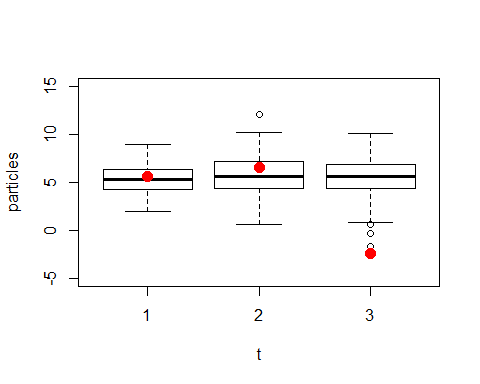
\includegraphics{meeting_report_5-27_files/figure-latex/unnamed-chunk-1-1.pdf}

\begin{Shaded}
\begin{Highlighting}[]
\NormalTok{fit <-}\StringTok{ }\KeywordTok{Arima}\NormalTok{(foo, }\DataTypeTok{order=}\KeywordTok{c}\NormalTok{(}\DecValTok{0}\NormalTok{,}\DecValTok{1}\NormalTok{,}\DecValTok{1}\NormalTok{), }\DataTypeTok{seasonal=}\KeywordTok{c}\NormalTok{(}\DecValTok{0}\NormalTok{,}\DecValTok{1}\NormalTok{,}\DecValTok{1}\NormalTok{))}
\KeywordTok{summary}\NormalTok{(fit)}
\end{Highlighting}
\end{Shaded}

\begin{verbatim}
## Series: foo 
## ARIMA(0,1,1)(0,1,1)[12] 
## 
## Coefficients:
##          ma1    sma1
##       0.4743  0.5398
## s.e.  0.0592  0.0519
## 
## sigma^2 estimated as 15.79:  log likelihood=-636.48
## AIC=1278.96   AICc=1279.07   BIC=1289.23
## 
## Training set error measures:
##                     ME     RMSE      MAE      MPE     MAPE       MASE
## Training set 0.2033584 3.847513 3.002382 0.661369 4.463736 0.03141502
##                     ACF1
## Training set -0.02291549
\end{verbatim}

\hypertarget{ii-reproduction}{%
\section{II Reproduction}\label{ii-reproduction}}

The main reference is the
\href{https://cran.r-project.org/web/packages/seasonal/vignettes/seas.pdf}{document}
about \emph{X-13ARIMA-SEATS(X-13)}. Something to clearify: By default, a
call to \textbf{seas} also invokes the following automatic procedures of
X-13: 1) Transformation selection (log / no log); 2) Detection of
trading day and Easter effects; 3) Outlier detection; 4) ARIMA model
search.

By default, seas calls the \emph{SEATS} adjustment procedure(which
decomposes the ARIMA model).To perform the alternative \emph{X-11}
adjustment procedure, we need to add \textbf{x11 = " "}.

But when I tried to use these code on the simulated data, the curves I
got from them are too smooth and looks same. I am thinking: maybe the
data I simulated before is not appropriate. In addition, something wrong
with the SEATS, cause the model from
it(\emph{SARIMA(0,1,1)(0,1,0){[}12{]}}) is different from that of x-11,
which is close to our true model \emph{SARIMA(0,1,1)(0,1,1){[}12{]}}

\begin{Shaded}
\begin{Highlighting}[]
\KeywordTok{library}\NormalTok{(seasonal)}
\KeywordTok{library}\NormalTok{(forecast)}
\KeywordTok{set.seed}\NormalTok{(}\DecValTok{1}\NormalTok{)}
\NormalTok{model <-}\StringTok{ }\KeywordTok{Arima}\NormalTok{(}\KeywordTok{ts}\NormalTok{(}\KeywordTok{rnorm}\NormalTok{(}\DecValTok{24000}\NormalTok{),}\DataTypeTok{freq=}\DecValTok{12}\NormalTok{), }\DataTypeTok{order=}\KeywordTok{c}\NormalTok{(}\DecValTok{0}\NormalTok{,}\DecValTok{1}\NormalTok{,}\DecValTok{1}\NormalTok{), }\DataTypeTok{seasonal=}\KeywordTok{c}\NormalTok{(}\DecValTok{0}\NormalTok{,}\DecValTok{1}\NormalTok{,}\DecValTok{1}\NormalTok{),}\DataTypeTok{fixed=}\KeywordTok{c}\NormalTok{(}\DataTypeTok{theta=}\FloatTok{0.5}\NormalTok{, }\DataTypeTok{Theta=}\FloatTok{0.5}\NormalTok{))}
\NormalTok{data <-}\StringTok{ }\KeywordTok{simulate}\NormalTok{(model,}\DataTypeTok{nsim=}\DecValTok{240}\NormalTok{)}
\KeywordTok{plot}\NormalTok{(data)}
\end{Highlighting}
\end{Shaded}

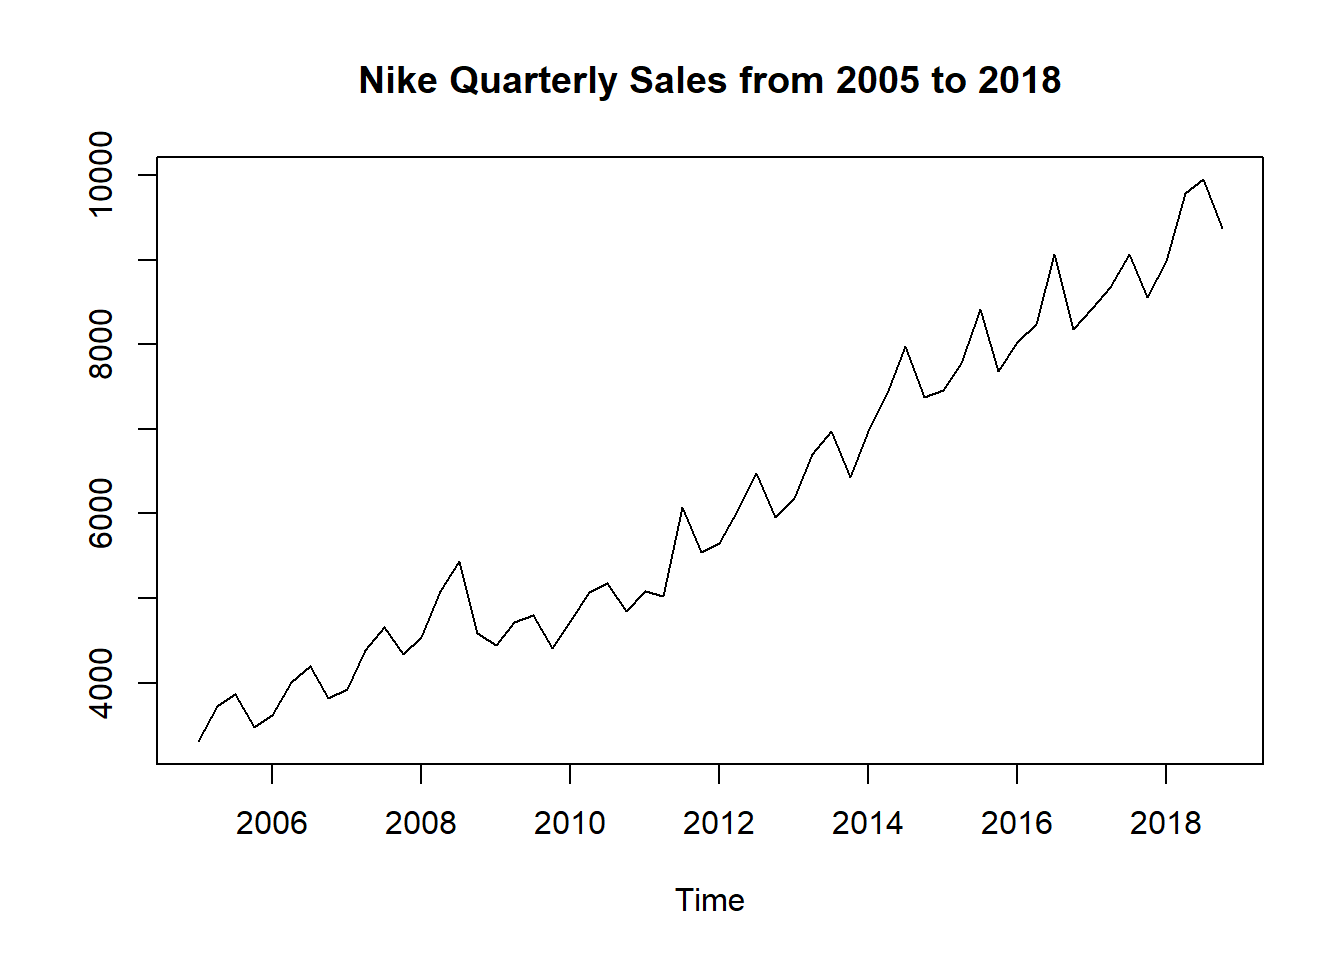
\includegraphics{meeting_report_5-27_files/figure-latex/unnamed-chunk-2-1.pdf}

\begin{Shaded}
\begin{Highlighting}[]
\NormalTok{m_x11 <-}\StringTok{ }\KeywordTok{seas}\NormalTok{(data, }\DataTypeTok{x11 =} \StringTok{""}\NormalTok{, }\DataTypeTok{regression.aictest =}  \OtherTok{NULL}\NormalTok{)}
\KeywordTok{plot}\NormalTok{(m_x11)}
\end{Highlighting}
\end{Shaded}

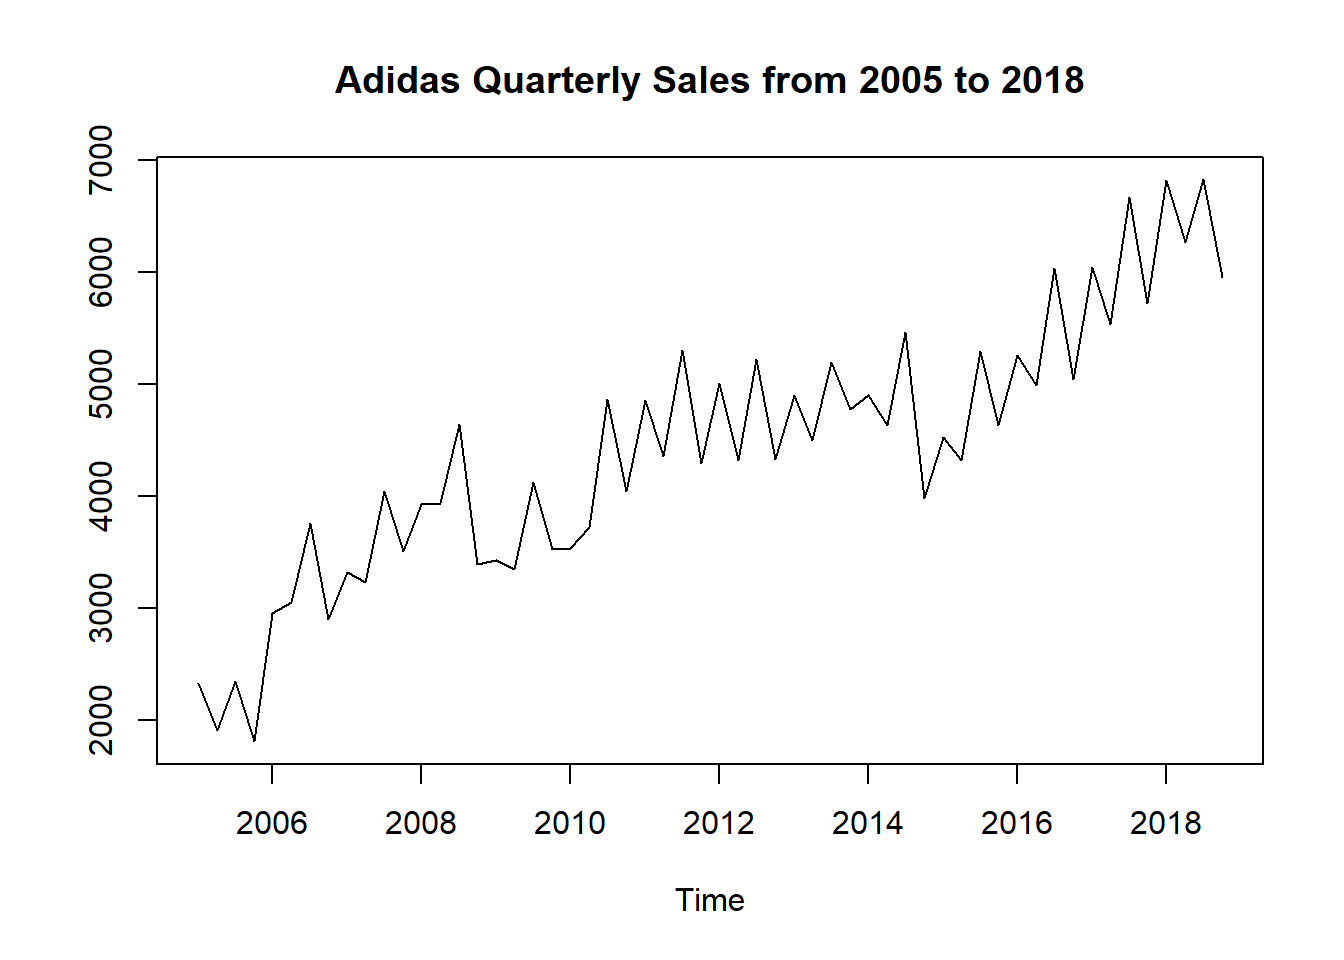
\includegraphics{meeting_report_5-27_files/figure-latex/unnamed-chunk-2-2.pdf}

\begin{Shaded}
\begin{Highlighting}[]
\NormalTok{m_seats <-}\StringTok{ }\KeywordTok{seas}\NormalTok{(data, }\DataTypeTok{regression.aictest =} \OtherTok{NULL}\NormalTok{)}
\end{Highlighting}
\end{Shaded}

\begin{verbatim}
## Model used in SEATS is different: (0 1 1)(0 1 0)
\end{verbatim}

\begin{Shaded}
\begin{Highlighting}[]
\KeywordTok{plot}\NormalTok{(m_seats)}
\end{Highlighting}
\end{Shaded}

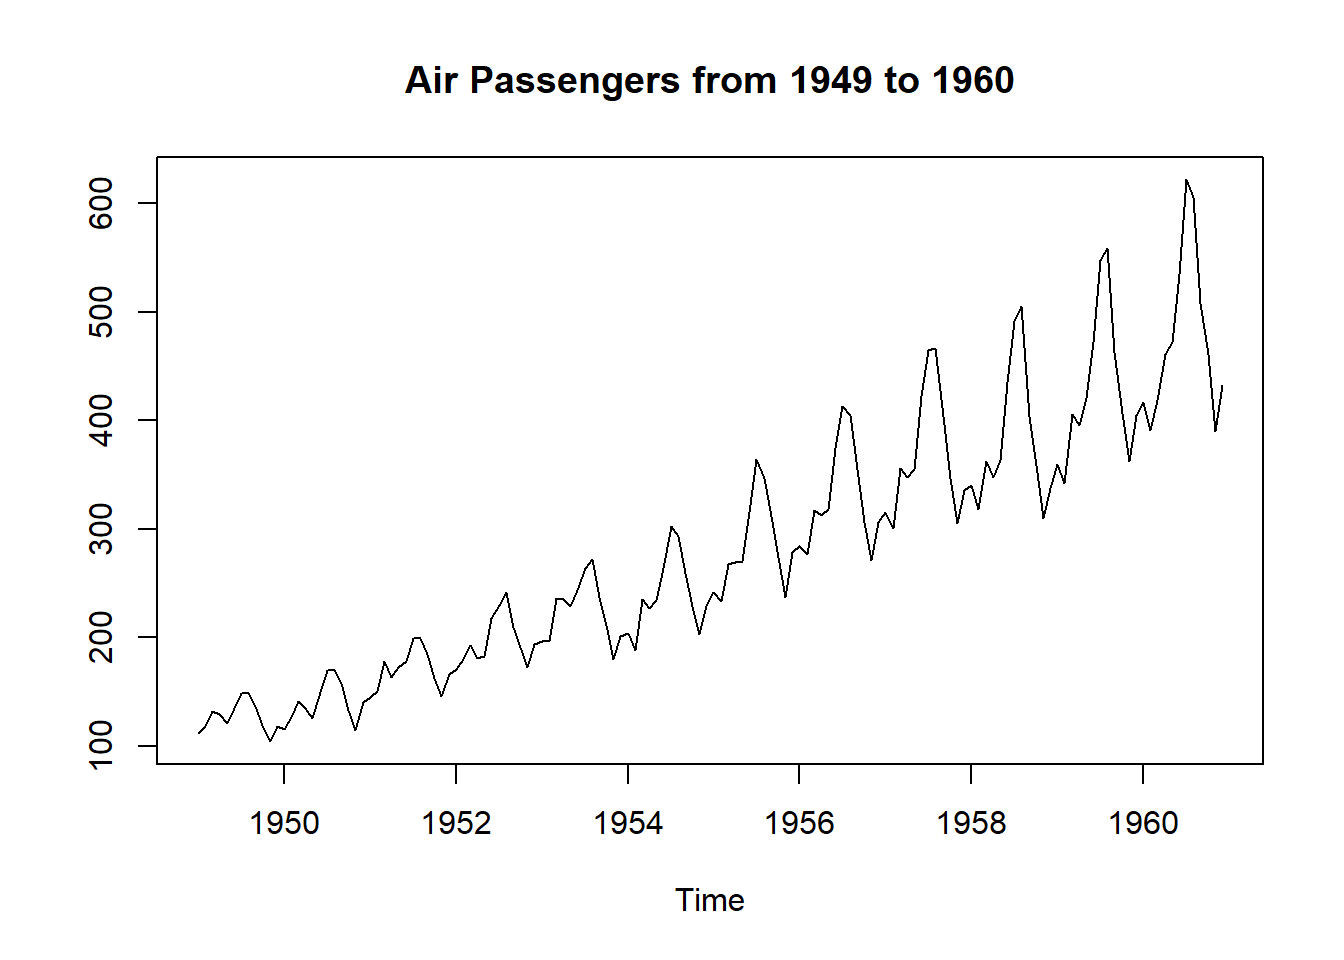
\includegraphics{meeting_report_5-27_files/figure-latex/unnamed-chunk-2-3.pdf}

\begin{Shaded}
\begin{Highlighting}[]
\KeywordTok{plot}\NormalTok{(data,}\DataTypeTok{col=}\StringTok{"green"}\NormalTok{,}\DataTypeTok{ylim=}\KeywordTok{c}\NormalTok{(}\OperatorTok{-}\DecValTok{10}\NormalTok{,}\DecValTok{2000}\NormalTok{),}\DataTypeTok{ylab=}\StringTok{""}\NormalTok{)}
\KeywordTok{par}\NormalTok{(}\DataTypeTok{new=}\NormalTok{T)}
\KeywordTok{plot}\NormalTok{(}\KeywordTok{final}\NormalTok{(m_x11),}\DataTypeTok{col=}\StringTok{"red"}\NormalTok{,}\DataTypeTok{ylim=}\KeywordTok{c}\NormalTok{(}\OperatorTok{-}\DecValTok{10}\NormalTok{,}\DecValTok{2000}\NormalTok{),}\DataTypeTok{ylab=}\StringTok{""}\NormalTok{)}
\KeywordTok{par}\NormalTok{(}\DataTypeTok{new=}\NormalTok{T)}
\KeywordTok{plot}\NormalTok{(}\KeywordTok{final}\NormalTok{(m_seats),}\DataTypeTok{col=}\StringTok{"blue"}\NormalTok{,}\DataTypeTok{ylim=}\KeywordTok{c}\NormalTok{(}\OperatorTok{-}\DecValTok{10}\NormalTok{,}\DecValTok{2000}\NormalTok{),}\DataTypeTok{ylab=}\StringTok{""}\NormalTok{)}
\KeywordTok{legend}\NormalTok{(}\StringTok{"topleft"}\NormalTok{,}\KeywordTok{c}\NormalTok{(}\StringTok{"Data"}\NormalTok{,}\StringTok{"X11"}\NormalTok{,}\StringTok{"SEATS"}\NormalTok{),}\DataTypeTok{col=}\KeywordTok{c}\NormalTok{(}\StringTok{"green"}\NormalTok{,}\StringTok{"red"}\NormalTok{,}\StringTok{"blue"}\NormalTok{),}\DataTypeTok{lty=}\KeywordTok{c}\NormalTok{(}\DecValTok{1}\NormalTok{,}\DecValTok{1}\NormalTok{,}\DecValTok{1}\NormalTok{))}
\end{Highlighting}
\end{Shaded}

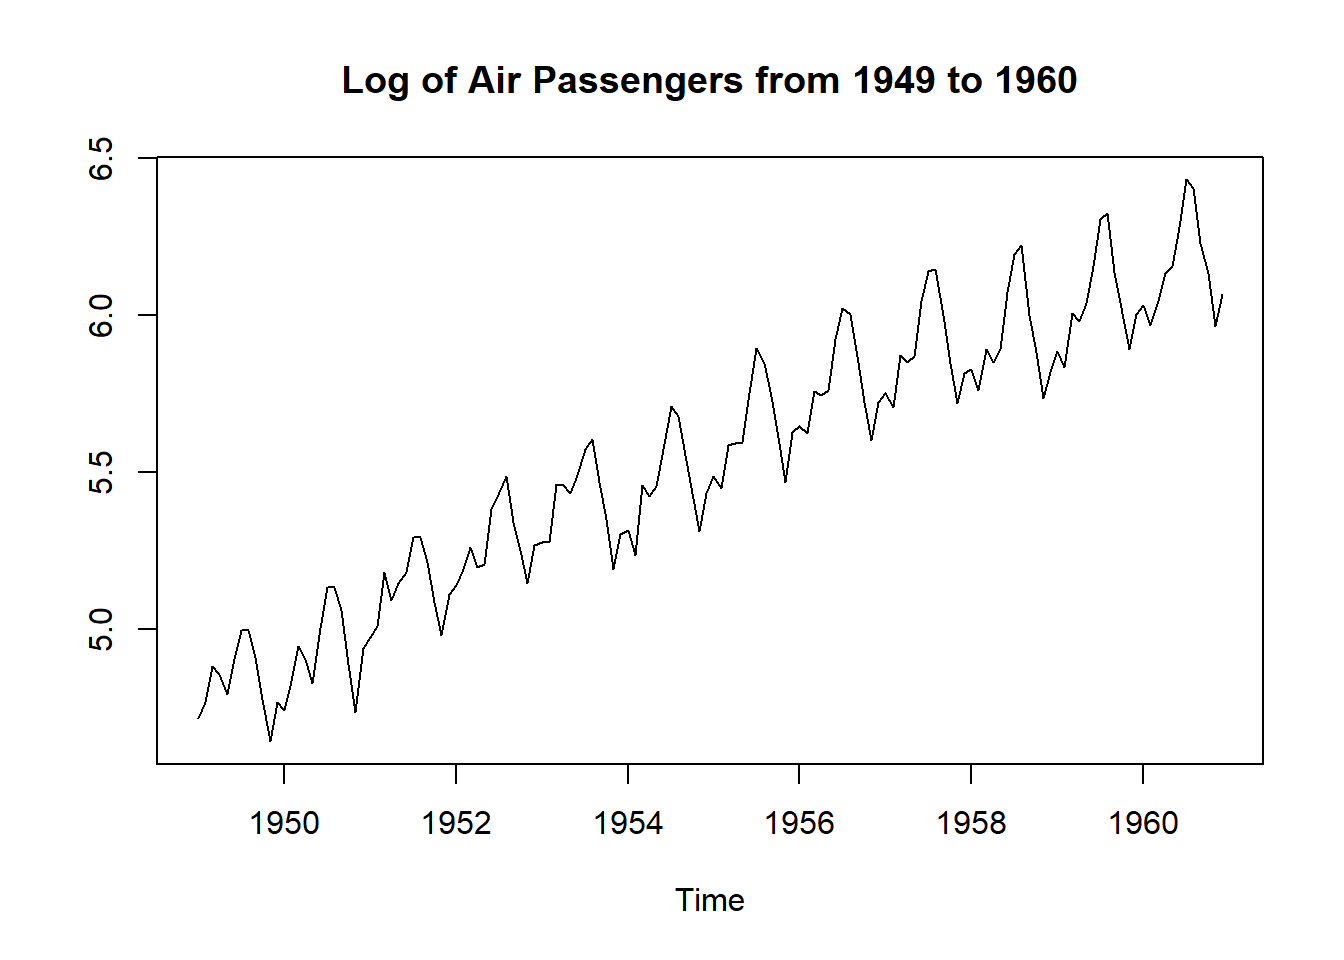
\includegraphics{meeting_report_5-27_files/figure-latex/unnamed-chunk-2-4.pdf}

I tried the same code on the data set \textbf{unemp}, whose results seem
to be good, at least not very smooth and not totally same:

\begin{Shaded}
\begin{Highlighting}[]
\KeywordTok{library}\NormalTok{(seasonal)}
\KeywordTok{library}\NormalTok{(seasonalview)}
\end{Highlighting}
\end{Shaded}

\begin{verbatim}
## 
## Attaching package: 'seasonalview'
\end{verbatim}

\begin{verbatim}
## The following object is masked from 'package:seasonal':
## 
##     view
\end{verbatim}

\begin{Shaded}
\begin{Highlighting}[]
\NormalTok{eg_seats <-}\StringTok{ }\KeywordTok{seas}\NormalTok{(unemp)}
\NormalTok{eg_x11 <-}\StringTok{ }\KeywordTok{seas}\NormalTok{(unemp, }\DataTypeTok{x11 =} \StringTok{""}\NormalTok{)}
\KeywordTok{plot}\NormalTok{(unemp,}\DataTypeTok{col=}\StringTok{"lightblue"}\NormalTok{,}\DataTypeTok{ylim=}\KeywordTok{c}\NormalTok{(}\DecValTok{5500}\NormalTok{,}\DecValTok{15300}\NormalTok{),}\DataTypeTok{ylab=}\StringTok{""}\NormalTok{)}
\KeywordTok{par}\NormalTok{(}\DataTypeTok{new=}\NormalTok{T)}
\KeywordTok{plot}\NormalTok{(}\KeywordTok{final}\NormalTok{(eg_seats),}\DataTypeTok{col=}\StringTok{"red"}\NormalTok{,}\DataTypeTok{ylim=}\KeywordTok{c}\NormalTok{(}\DecValTok{5500}\NormalTok{,}\DecValTok{15300}\NormalTok{),}\DataTypeTok{ylab=}\StringTok{""}\NormalTok{)}
\KeywordTok{par}\NormalTok{(}\DataTypeTok{new=}\NormalTok{T)}
\KeywordTok{plot}\NormalTok{(}\KeywordTok{final}\NormalTok{(eg_x11),}\DataTypeTok{col=}\StringTok{"blue"}\NormalTok{,}\DataTypeTok{ylim=}\KeywordTok{c}\NormalTok{(}\DecValTok{5500}\NormalTok{,}\DecValTok{15300}\NormalTok{),}\DataTypeTok{ylab=}\StringTok{""}\NormalTok{)}
\end{Highlighting}
\end{Shaded}

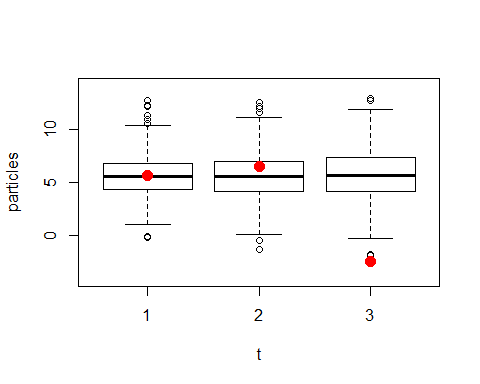
\includegraphics{meeting_report_5-27_files/figure-latex/unnamed-chunk-3-1.pdf}

And I am still working on the state space model.

\textbf{Update 5.30} 以下是Aaron的回复,包含了几条不错的建议: *
对spickness的讨论不够


\end{document}
